% Kinematic fitting at ANKE
Разработанное расширение было использовано авторами для кинематического фита в реакции $pp \to pp$ на данных, полученных на спектрометре ANKE (Jülich, Germany) [TODO: вставить ссылку на ANKE].

На рисунке \eqref{anke_scheme} можно видеть, что в процессе прохождения протонного пучка через установку часть протонов может отклоняться от направления основного пучка и не фиксироваться установкой, таким образом при анализе данных эксперимента мы можем столкнуться с разницей зафиксированных энергий и количества вещества, вступившего в реакцию с данными, полученными на выходе. Восстановить долю таких ``потерянных'' протонов мы можем, используя инвариант Лоренца $\left|\boldsymbol{P}^{(4)}_\mathrm{beam}+\boldsymbol{P}^{(4)}_\mathrm{targ}-\boldsymbol{P}^{(4)}_p\right|^2 = m_p^2$.

TODO: Добавить, причем тут Polar CMS coordinates.

\begin{figure}[h]
\centering
\centering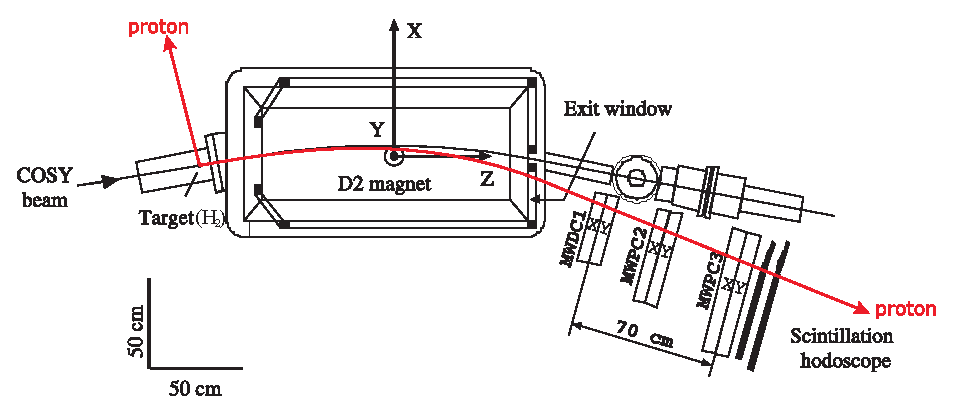
\includegraphics[width=0.8\textwidth]{pics/setup_.eps}
\caption{
Схема прохождения протонного пучка через установку ANKE.
}
\label{anke_scheme}
\end{figure}

% \centering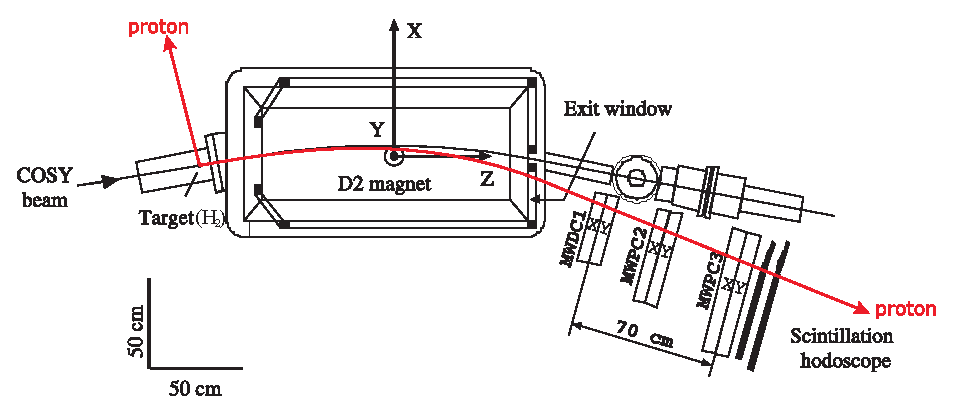
\includegraphics[width=0.8\textwidth]{pics/setup_.eps}

% \large
% \phantom{0}
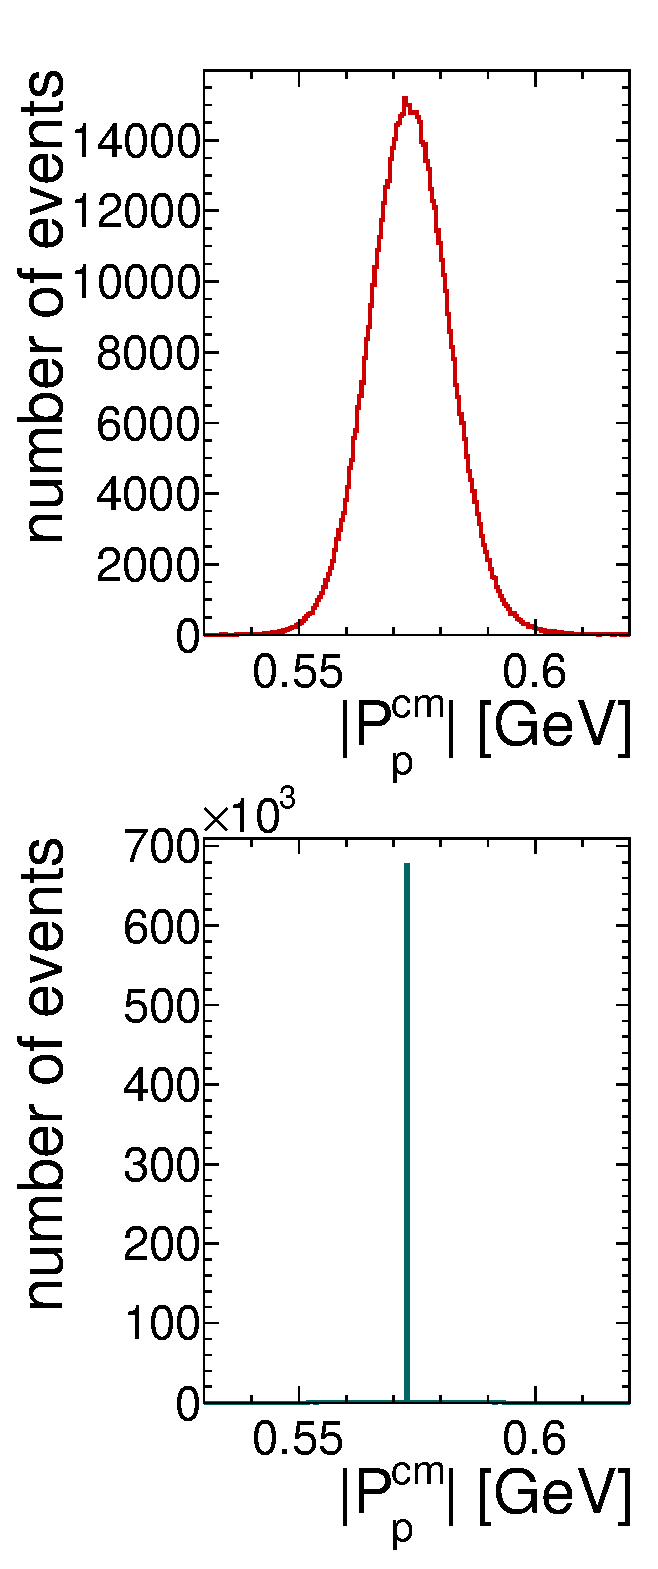
\includegraphics[height=0.7\textheight]{pics/drawMom.eps}
\hfill
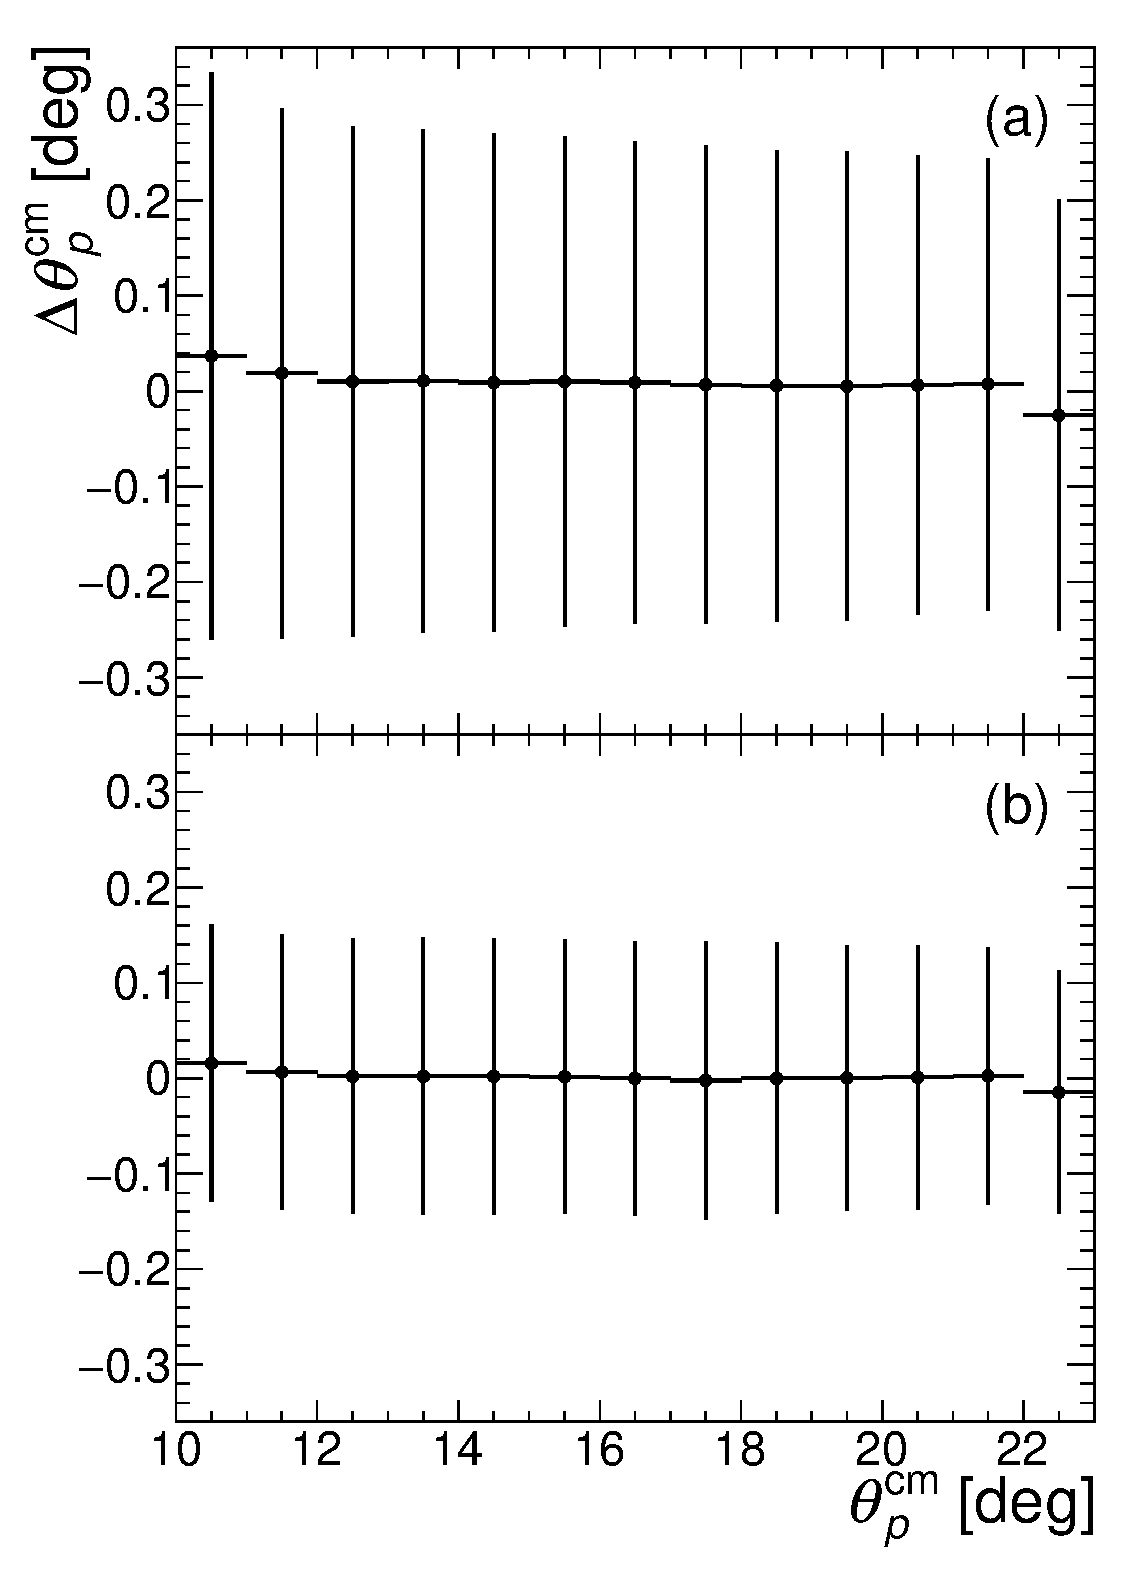
\includegraphics[height=0.7\textheight]{pics/drawTh.eps}
\hfill
% \hspace{1em}
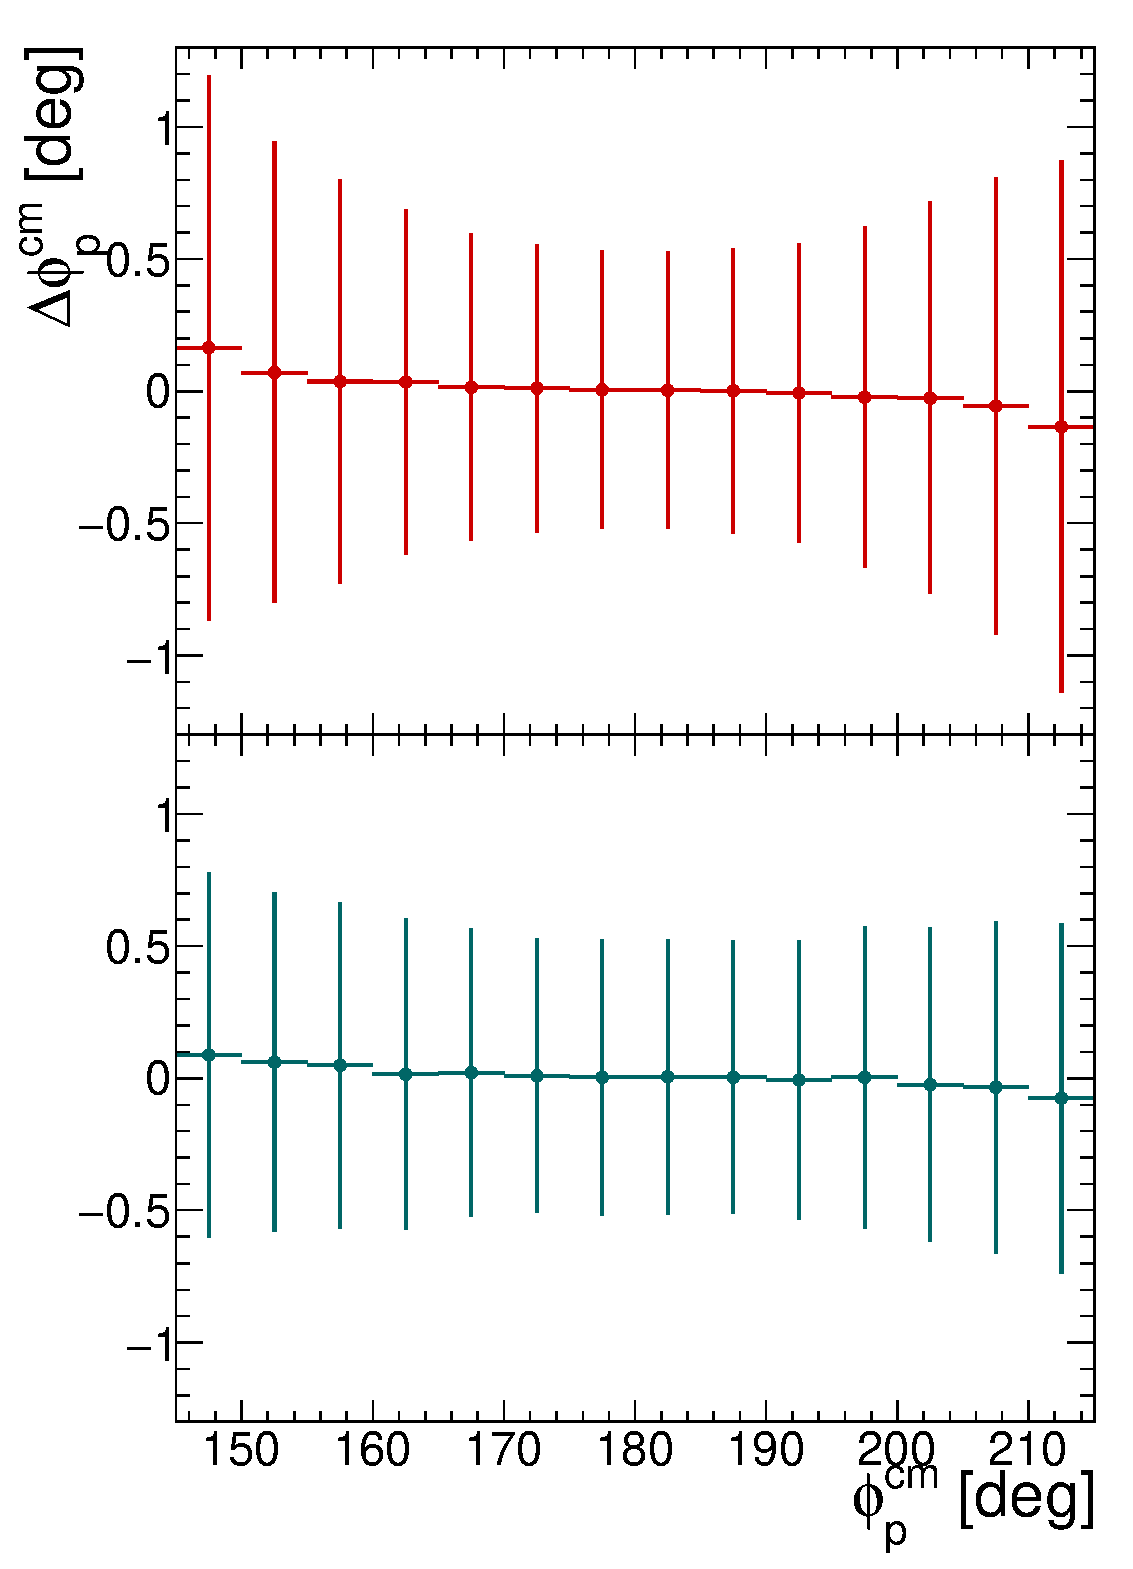
\includegraphics[height=0.7\textheight]{pics/drawPhi.eps}
% \hfill
% \phantom{0}

Errors of reconstructed proton momentum in polar coordinates $(|P_p^\mathrm{cm}|, \theta_p^\mathrm{cm}, \phi_p^\mathrm{cm})$ for the $pp \to pp$ reaction at ANKE, simulated for $T_\mathrm{beam} = 700$~MeV with and without kinematic fitting.
